%----------------------------------------------------------------------------------------
%	DATA ACQUISITION AND PREPARATIONS
%----------------------------------------------------------------------------------------

\section{Data acquisition and organization}
\label{ch:DataAcquisition}

The first section of the chapter~\ref{sec:Roadmap}~\nameref{sec:Roadmap} gives an overview of the time management of the study group. It is followed by the subchapter~\ref{sec:Organization}~\nameref{sec:Organization} in which communication and teamwork are assessed. In~\ref{sec:DataCollection} \nameref{sec:DataCollection}, the acquisition of the data from the sorting machine Autoselect ATS~II is described in more detail. The last section~\ref{sec:Literature}~\nameref{sec:Literature} presents the retrieved literature concerning the issue of asparagus classification and agricultural product classification with machine learning based approaches.

\subsection{Roadmap of the project}
\label{sec:Roadmap}

At the beginning of the project, a roadmap was created to structure the year into different working stages as well as to have an overview of the tasks and problems that needed to be addressed.

\begin{figure}[h]
	\centering
	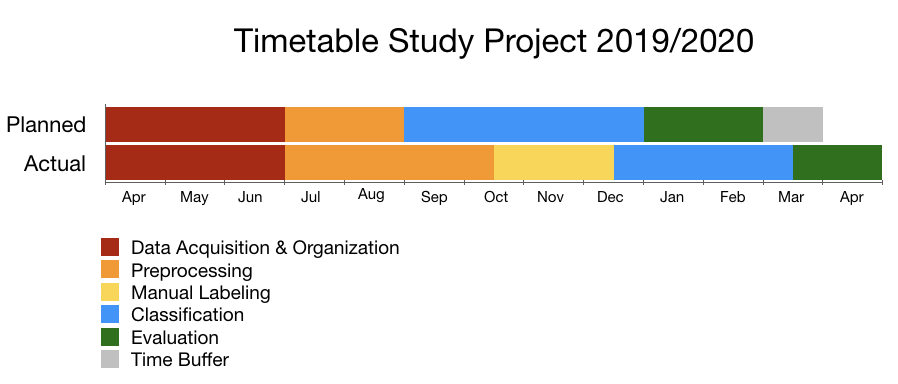
\includegraphics[scale=0.43]{Figures/chapter02/new_timetable.png}
	\decoRule
	\caption[Timetable of the Project]{\textbf{Timetable of the Project}~~~The upper timeline shows the estimated time of the study project from April 2019 to April/Mai 2020. The lower timeline displays how the time was spent. Both timelines differ in that the year was more optimistically planned than realized. A major factor was the lack of experience of the participants concerning the conduction of a larger project with many co-workers as well as concerning the general implementation of the preprocessing stage for machine learning classification. Another factor influencing the shifted timeline was the appearance of a fifth major stage, the \emph{Manual Labeling}.}
	\label{fig:Timetable}
\end{figure}

\begin{figure}[h]
	\centering
	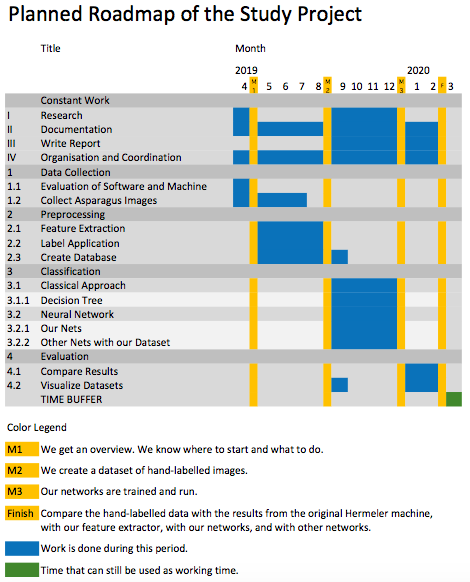
\includegraphics[scale=0.7]{Figures/chapter02/roadmap_planned.png}
	\decoRule
	\caption[Planned Roadmap]{\textbf{Planned Roadmap}~~~The figure shows the planned roadmap of the study project. It reveals how the time needed for each task was estimated in the beginning of the project.}
	\label{fig:RoadmapPlanned}
\end{figure}

\begin{figure}[h]
	\centering
	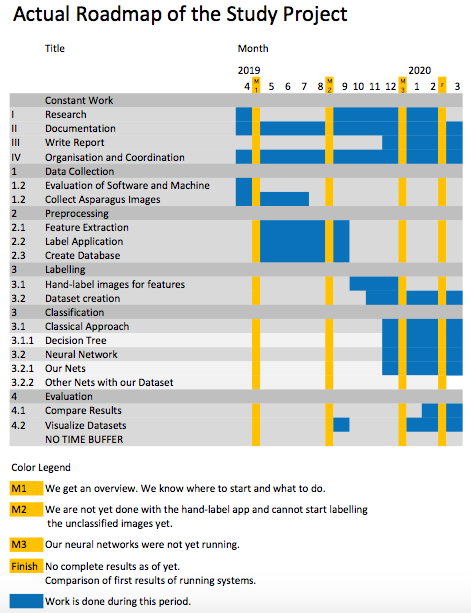
\includegraphics[scale=0.7]{Figures/chapter02/roadmap_actual.png}
	\decoRule
	\caption[Actual Roadmap]{\textbf{Actual Roadmap}~~~A roadmap that shows how the time was spent.}
	\label{fig:RoadmapActual}
\end{figure}

The timetable in~\autoref{fig:Timetable} gives a broad outline of the major stages of the project. In the upper timeline of the figure, it was estimated how much time for a specific phase is needed, whereas in the lower timeline the time spent for the stage is given. Both timelines are structured to display the project year, starting in April 2019 and ending in April/Mai 2020. The months are represented by the x-axis while the colors mark the different working stages.

The project comprises four to five major stages: \textit{Data Collection \& Organization}, \textit{Preprocessing}, \textit{Manual Labeling}, \textit{Classification}, and \textit{Evaluation}. A detailed representation of the single tasks attributed to each stage can be found in the roadmaps in~\autoref{fig:RoadmapPlanned} and~\autoref{fig:RoadmapActual}. The project started with the data collection and the organization of the study project. During the first stage, the images were recorded with the sorting machine, while the major planning and research for the project took place. In the second phase, most of the preprocessing happened, that is, preparing and labeling the image data. The classification stage includes the time spent on the machine learning approaches which were implemented and trained on the asparagus data. In the last stage, the approaches were evaluated and their results were compared. The different stages overlapped to a certain degree. For the purpose of this figure, the start and end time is displayed as a hard boundary.

When comparing both timelines, some distinctions can be recognized. The upper timeline shows that preprocessing was estimated to be done by September. However, the phase continued until October, as can be observed in the lower timeline. Furthermore, the time for labeling a sufficient amount of images was underestimated, resulting in adjustments of the time attributed to this task. More specifically, it led to the \textit{Manual Labeling} of the image data receiving its own phase in the timetable, independent of the preprocessing phase.

The differences are depicted with different color codings. While the main focus of this project was supposed to be the application of different machine learning techniques to classify the data (color-coded in blue and green), the preprocessing phase and the data set creation/manual labeling posed to be most time-consuming (color-coded in orange and yellow).

In~\autoref{fig:RoadmapPlanned} and~\autoref{fig:RoadmapActual}, the stage specific tasks can be seen in more detail. Again, both figures display the estimated time and the actual time, respectively. The headlines serve as a division into the major stages except for the first heading, \emph{Constant Work}, which shows the tasks that demanded continuous attention and effort throughout the year. The duration of tasks is represented in blue, while the yellow lines mark milestones that are explained in the legends.

\subsection{Organisation of the study group}
\label{sec:Organization}

In this chapter, the management of the work distribution and the communication are taken into focus. For this the tools that were used for communication and organization will be examined as well as the structure of the group work.


\subsubsection{Communication}
\label{subsec:Communication}

The main communication consisted of weekly meetings in which the working process was discussed and new tasks were distributed. In addition to those meetings, different platforms were used, which worked with varying degrees of success. Used platforms were Asana, GitHub and Telegram to facilitate the communication aside from group meetings. The different means of communication will be described and evaluated in the following abstract.

\bigskip
Regular meetings have been the most helpful in organizing our project. During the meetings, which usually lasted from one to two hours, a discussion leader and a protocol writer were picked. The protocols were saved for review in the GitHub project.\footnote{ see~\url{https://github.com/CogSciUOS/asparagus}} The meetings were characterized by long discussions about the best approach for the following steps and further possibilities to tackle the next challenge. The project’s supervisors were usually present at the meetings, to bring in their expertise and to give the opportunity to ask concrete questions. During the first half of the project, tasks were always distributed at the end of each meeting. In the following meeting the progress of the work was discussed. This procedure was changed in the second half of the project. We started to use a schedule that described the different tasks and deadlines in detail. Additionally, we regularly gathered for co-working. The organizational meetings were continued, during which everyone gave precise and structured reports on their area of responsibility. This helped us to spend less time discussing and debating and more time working on our tasks.

Telegram is a cloud-based instant messaging service for the use on smartphones, tablets and computers. Starting from the first meeting, we had a constant conversation in a group chat on Telegram, in which we informed each other about the status of the project as well as support each other by answering questions. The group chat also created space for mutual motivation when needed. The majority of important information was exchanged via telegram.

Asana is used to distribute tasks and to communicate projects successfully. Many integrations of other applications, such as Slack, can help to achieve this. We used a board view where we listed tasks in different sections. But this function alone did not help us much in our project. The tasks were easier to distribute in direct consultation at physical meetings and demonstrated or discussed after completion. So it happened that Asana was not used enough to be helpful. If we had relied on communication with Slack or other agreed services or applications, it might have made more sense, but Asana alone was proven to be inefficient in our use case.

GitHub is a web-based popular platform using the version control system Git that helps developers to store and manage their code, and track and control changes to their project. During the project, we learned how to use it. Git allowed us to work from anywhere, which encouraged the workflow. Furthermore, we were able to automatically create a documentation via Sphinx. This means that by adhering to the style conventions, the protocols, work schedules, manuals, and code comments were automatically deployed as our documentation.\footnote{see~\url{https://asparagus.readthedocs.io/en/latest/}}


\subsubsection{Teamwork}
\label{subsec:Teamwork}

This subchapter starts by introducing the team members and our previous experiences. This is followed by a description of the practical aspects of teamwork, the work structure, and the distribution of project-relevant tasks.

\bigskip
The project was an initiative of one of the students and, hence, a large part of the project members knew each other from their private environment but had not yet worked together. Further students joined the project after its public announcement to complete the team. Thus, the group consisted of members with varying degrees of knowledge about each other. The team was initially made up by Malin Spaniol, Maren Born, Katharina Groß, Josefine Zerbe, Michael Gerstenberger, Richard Ruppel, Sophia Schulze-Weddige, Luana Vaduva, Thomas Klein and Subir Das. None of the members had yet worked together as such on a project of this scope. During the course of the project, three members left the team for various reasons. Thomas left in July due to a change in his study program. This was an unfortunate occurrence because he posed a valuable source of knowledge in the field of computer vision. Further, Luana and Subir left in October to pursue different study projects.

\bigskip
The members brought a wide variety of backgrounds into the team through different bachelor programs or different majors in the broader field of Cognitive Science. In the beginning of the project, the team members had little to no experience in the application of computer vision or neural networks. The motivation of most students was to pursue new and interesting tasks in these fields. Four students had a theoretical background in computer vision, six students had gained some experience with neural networks through the course ``\acrshortpl{ann} with Tensorflow’’, taught at the University of Osnabr{\"u}ck, while some had also taken machine learning classes during their study program. None of the members had prior knowledge about project management or task organization on a broader level. Git was previously only used by three students so far, but none of them were experts on its usage. Further, participants had neither experience with the Grid system of the \acrshort{ikw}, nor with running jobs on different machines. Thus, the project started with ten members, each of them with a different level of experience in the most relevant fields of machine learning, that is computer vision and neural networks.

\bigskip
As none of the members had any previous experience with team formation, the team lacked some structure and a clear distribution of individual roles in the beginning. One reason for this could have been the harmonious atmosphere between team members due to their friendship. Further tasks such as the trips to the asparagus farm strengthened the team spirit and the social interactions. We therefore started with a very dynamic structuring of tasks distribution by making every decision democratically. Most tasks were done in smaller teams of two to three people. Rather few tasks were done alone. In our meetings, we often formulated possible next tasks, even for the distant future, but  without assigning them to specific persons or working groups. This resulted in a lot of unassigned tasks and a discontinuous workflow. 

In August, we restructured our own organization. On the one hand, this was due to the fact that the tasks changed and thus a new structure was more appropriate. On the other hand, the strengths of the individual team members were a reason for the restructuring. Some team members had less programming experience than others and therefore had difficulties realizing certain tasks in an equal time period and with the same precision as others. Even if they had good ideas in terms of concept, it was not possible for them to implement these ideas quickly enough so that they could be included into the project. Nevertheless, there was still the possibility to grow skills in new assignments. In addition, the democratic self-organization and difference in programming expertise led to a distortion in the time management of the group and some tasks were not finished in time. To integrate more of the strengths that the single team members brought and to tackle the issue of time management, it was decided to write a work schedule that distributed the work more appropriately, gave an overview of the tasks that still had to be done and how much time was left to do them.

Further, common working hours on campus were introduced. In addition, the responsibilities were shared for both, work tasks and the supervision of those work tasks. The common working hours ensured that questions and decisions that arose could be discussed in person. This was especially helpful when different tasks overlapped and required communication and agreement.

The supervision of the work was divided into manager roles, which means that the work was split into different main fields where each member was responsible for managing their assigned area, distributing tasks and keeping an overview of the relevant work inside their working field. Furthermore, one knew who to consult for questions  in need of discussion or feedback. The meetings became more effective due to the new structure, and there was less discussion concerning task distribution. As we distributed roles, we were also more responsive to the strengths and weaknesses of the group members. Therefore one can say that the team structure and distribution of work changed over the course of the project. The strengths of single members were used more efficiently and the supervision of working areas led to a more structured supervision and task distribution. 


\subsection{Data collection}
\label{sec:DataCollection}

First, the asparagus sorting machine at Gut Holsterfeld is described before reporting about the process of labeled and unlabeled data collection.

The machine Autoselect ATS~II (2003) is designed for sorting white and green asparagus~\citep{autoselectanleitung}(see~\autoref{fig:SortingMachine}). The asparagus is arranged on a conveyor belt that runs it through the recording section of the machine. Here, a camera takes three pictures per asparagus (see \autoref{fig:SortingMachineSketch} and \autoref{fig:ExampleImagesAnna}). Small wheels on the conveyor belt rotate the asparagus in the meantime so that it can be photographed from several positions. In the best case, on each image a different side of the asparagus is recorded. The conveyor belt transports the spear further and it is sorted into a tray depending on the chosen class label by the machine. The sorting is based on the parameters width, length, shape, curvature, rust, and color. A total of 30 criteria for classifying an asparagus spear are used to describe these parameters. The calculation of the single features is based on a classical analytical approach. For example, the feature color is composed of eight sub-parameters. Each spear is reviewed at different areas (the head of the asparagus, the area below the head, and the stem) and judged for its hue in percentage. The values are compared and, according to a threshold, the spear is sorted into a color category. For all parameters, there is a minimal threshold and a maximal threshold. As another example, the parameter width is calculated at three points at the asparagus (top, middle, and bottom part). From these three values, an average value is calculated that decides in which category the asparagus is sorted. If an asparagus exceeds the maximal threshold, it is not recognized and cannot be sorted accordingly. Thus, all parameters have to have an upper and a lower threshold, including parameters like shape, curvature, and color. When evaluating which thresholds to choose, it is recommended to check that most asparagus spears tend to be in between the average value and the maximal threshold, with a larger tendency to accumulate around the average value. All parameters can be freely chosen by the farmer and can in this way be fitted to the needs of the respective asparagus farm.

\begin{figure}[!htb]
	\centering
	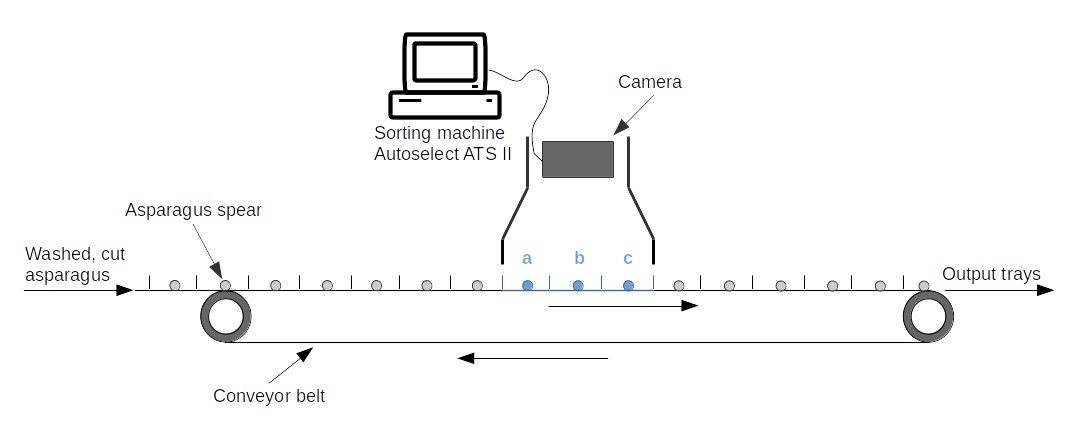
\includegraphics[width=0.9\textwidth]{Figures/chapter02/asparagusconveyerbelt_new.png}
	\decoRule
	\caption[Sketch of the Image Capturing Process with the Autoselect ATS II]{\textbf{Sketch of the Image Capturing Process with the Autoselect ATS II}~~~The asparagus spears are transported on a conveyor belt. After being washed and cut, the spears pass the camera field. Images are taken of three compartments, so that each asparagus spear is photographed three times in each position (a, b, c). The camera system is connected to a computer on which the sorting software runs. Depending on the resulting classification, the spear is sorted into the corresponding output tray.}
	\label{fig:SortingMachineSketch}
	\vspace{15pt}
	\centering
	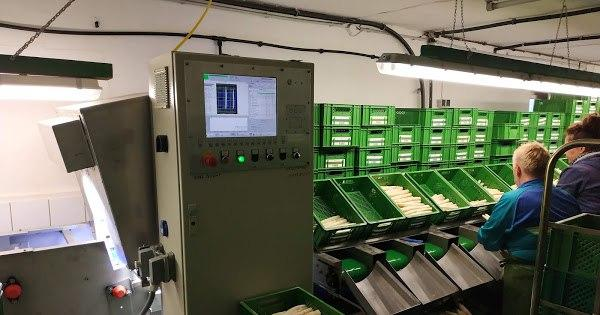
\includegraphics[scale=0.6]{Figures/chapter02/sortingmachine_front.png}
	\decoRule
	\caption[The Autoselect ATS II at Gut Holsterfeld]{\textbf{Autoselect ATS~II at Gut Holsterfeld}~~~In the figure the asparagus sorting machine Autoselect ATS~II at Gut Holsterfeld can be seen. The conveyor belt transports the asparagus from the left side of the image to the right side. It thereby passes the camera system. The display of the machine gives information on the parameters and the images. The machine is mainly controlled from here.}
	\label{fig:SortingMachine}
\end{figure}

\begin{figure}[h]
	\centering
	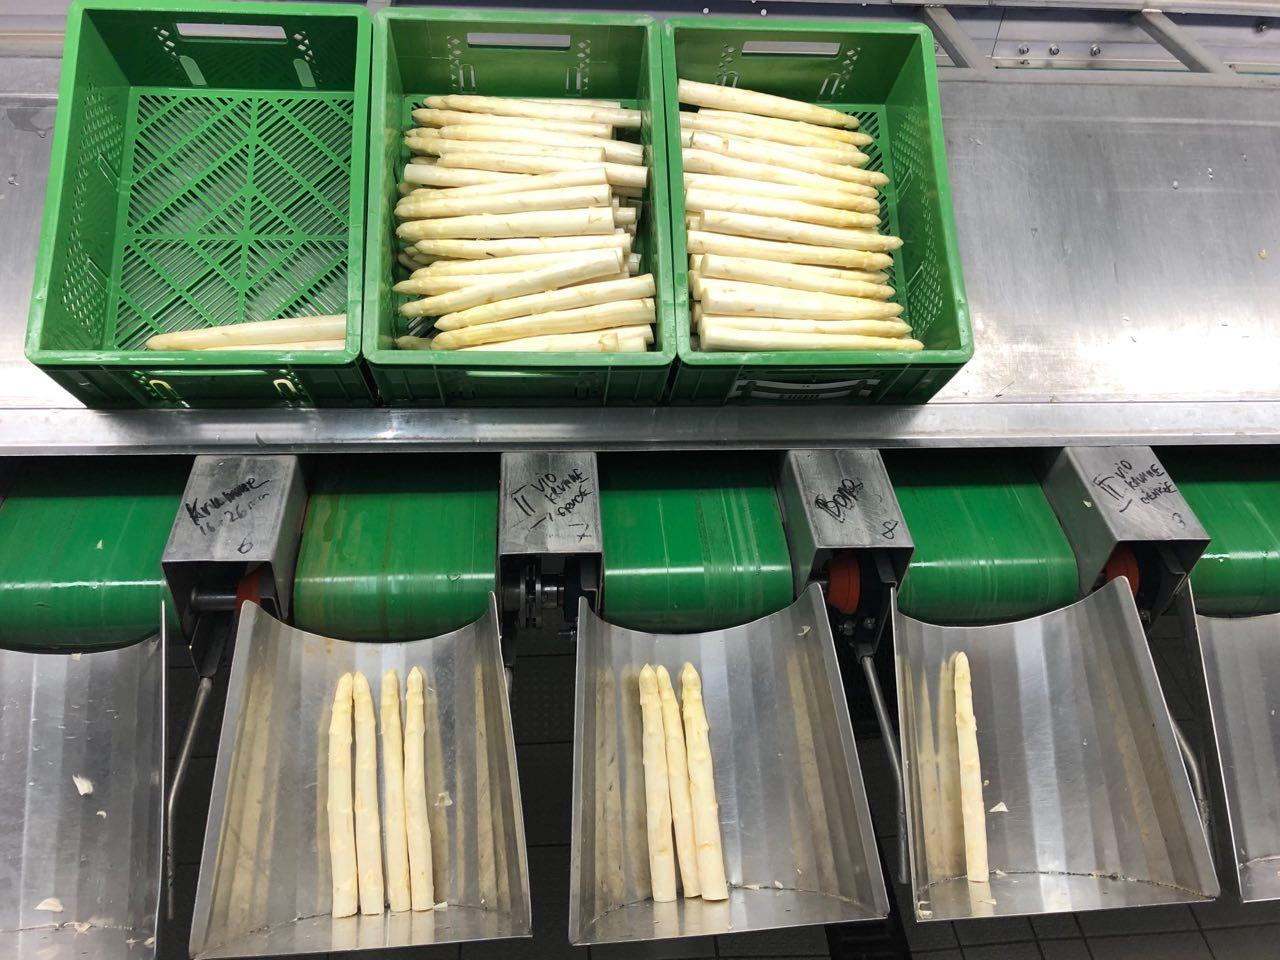
\includegraphics[scale=0.3]{Figures/chapter02/sorting_machine_slots.png}
	\decoRule
	\caption[Output Trays of the Sorting Machine]{\textbf{Output Trays of the Sorting Machine}~~~Depending on the class label, the asparagus is sorted into one of the machine's 16 trays.}
	\label{fig:SortingMachineSlots}
\end{figure}

According to the manual, the number of quality classes is selectable but limited by the number of output trays available to the machine. The machine Autoselect ATS~II at Gut Holsterfeld has 16 trays (see~\autoref{fig:SortingMachineSlots}). The user can define the order of parameters. The manufacturer suggests to first sort for length and width, then sort for colors parameters, and analyze the shape parameters last.

Before the first use of the machine, all parameters are selected after a calibrating charge of asparagus has run through the machine. Then, the user can adjust the thresholds accordingly.

The accuracy of the sorting machine is described to be as good as 90\% best case by the manufacturer, while the farmer at Gut Holsterfeld reported it to be around 70\% at best, with re-sorting being necessary by professional sorters. Especially categories like Blume or Hohle were considered to be inconsistent by both, manufacturer and farmer. Further information could not be given on the software of the machine. A meeting with a representative of the engineering company HMF that manufactured the sorting machine was arranged.~\footnote{ see \url{www.hmf-hermeler.de}} Unfortunately, the source code itself was not available to HMF as it was produced by another company. 

\bigskip
In the following it is described how the image data was collected. It is possible to save images with the Autoselect ATS~II, however, the storage space on the machine is very limited. Further, the selection of images to be saved is restricted to only 1000 images.
One workaround to the problem is the installation of the Teamviewer software on the machine and the connection of an external hard drive. After the installation, the process of image collection could be started remotely. This work was very ineffective and time-consuming. The data could not be directly transmitted to another computer because the internet connection at the farm is too slow. An automatic transfer of the images to the external hard drive was not possible until the installation of an automatic file moving service, for which the requirements are described below.

The file moving program needs to transfer the images to a new saving destination and has to run in the background without disturbing the workflow of the sorting machine. After research on background processes and programs, the decision was made to use a service, that is, a system process running independently of any program. As Windows is used as the operating system of the sorting machine, the development was done with the .NET framework in the programming language C\#. The package provided is called Topshelf.\footnote{For further information on Topshelf, see \url{https://github.com/Topshelf/Topshelf}.} Topshelf is a service hosting framework for building Windows services using .NET.\footnote{For further information on the .NET framework, see \url{https://docs.microsoft.com/en-us/dotnet/framework/get-started/overview}.} With the package, it is possible to develop a console application in the development phase, compile it as a service, and install it later via the console. Previously, it was not possible to debug services during the development phase. The function of the service is based on the FileSystemWatcher object from the System.IO namespace.\footnote{For further information on the SystemFileWatcher, see \url{https://docs.microsoft.com/en-us/dotnet/api/system.io.filesystemwatcher?view=netframework-4.8}.} In the main program, a list of files in the source folder is kept. Files that are older than one hour are moved to the target folder on the external drive. The selected files are moved by a function that is called, when an event is triggered. The event is triggered by the FileSystemWatcher after subscribing to different flags. Shortly after initialization, the service was adjusted because removing the images from the C disk straight away caused the sorting program to stop. The problem is solved by keeping the most recent 1000 images and moving older images to the external disk.

\bigskip
The project members split in groups of two and exchanged the hard drive two times a week. The collected images were then transferred to storage capacities of the university.

Before the project had started, the farm had not collected any labeled data such that relying on the labels that the machine attributes to each asparagus is not possible. A solution is to send the already sorted asparagus a second time through the machine. Like this, it was assumed that not only labeled data can be acquired but also the parameters calculated by the machine. Unfortunately, it is not possible to extract the parameters from the machine. Another issue poses the fact that a second sorting is not good for the quality of the asparagus. Further, at least one project member has to be involved in the re-sorting and, thus, has to be present at the farm. The sessions of exchanging the external hard drive and collecting labeled image data were then combined.

\begin{figure}[h]
	\centering
	\vspace{20pt}
	\begin{subfigure}{0.3\textwidth}
		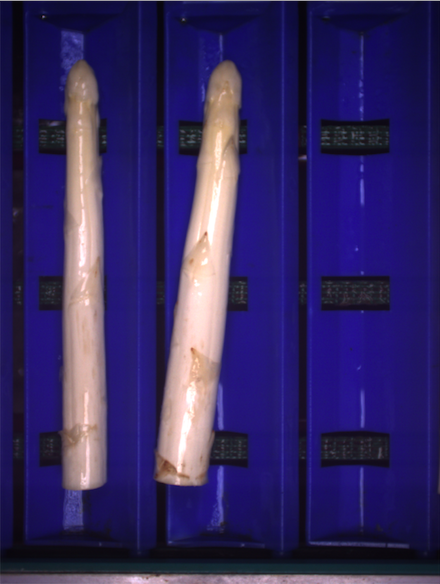
\includegraphics[width=0.95\linewidth]{Figures/chapter02/anna_a.png}
		\caption{left}
	\end{subfigure}
	\begin{subfigure}{0.3\textwidth}
		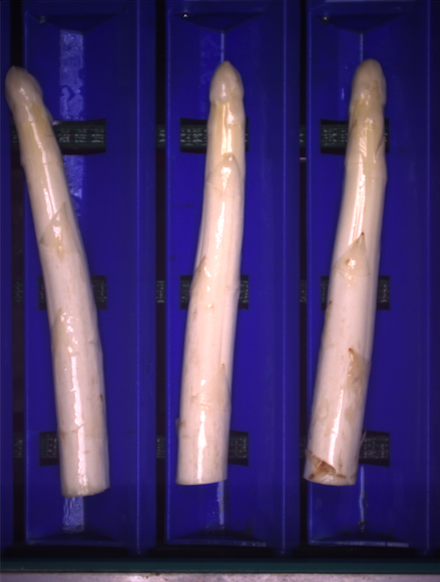
\includegraphics[width=0.95\linewidth]{Figures/chapter02/anna_b.png}
		\caption{middle}
	\end{subfigure}
	\begin{subfigure}{0.3\textwidth}
		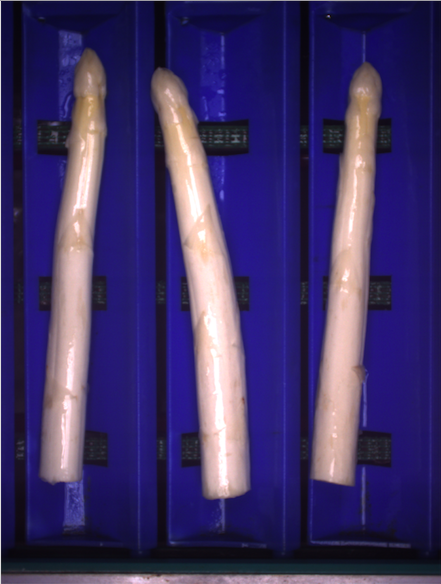
\includegraphics[width=0.95\linewidth]{Figures/chapter02/anna_c.png}
		\caption{right}
	\end{subfigure}
    \caption[Example Asparagus Images]{\textbf{Example Asparagus Images}~~~Example pictures of the quality class I~A~Anna. The asparagus is arranged on a conveyor belt that runs it through the recording section of the machine, where a camera takes three pictures. In picture (A) the asparagus is to the left, in (B) it is in the middle, and in (C) it is to the right. Small wheels on the conveyor belt rotate the asparagus in the meantime so that it can be photographed from several positions. In the best case, on each image a different side of the asparagus is recorded. The conveyor belt transports the spear further and it is sorted into a tray depending on the chosen quality class by the machine. 
}
    \label{fig:ExampleImagesAnna}
\end{figure}

\bigskip
An example image of the received data can be seen in~\autoref{fig:ExampleImagesAnna}. There are three pictures per asparagus. The image resolution is $1040\times1376$ pixel per image, with an RGB color space.

In total, 612113 images were collected, with each class label being represented with at least 309 images, corresponding to 103 asparagus.

At the asparagus farm Gut Holsterfeld, 591495 labeled and unlabeled images were collected with the Autoselect ATS~II. The number of unlabeled data is 578226 images, thus, around 192742 different asparagus spears. Of the labeled data, we collected 1005 images with the label I~A~Anna,  908 images for I~A~Bona, 513 images of I~A~Clara, 936 images of I~A~Krumme, 1514 images of I~A~Violett, 1051 images of II~A, 1468 images of II~B, 1169 images of Rost, 749 images of Dicke, 775 images of Hohle, 1717 images of Blume, 1157 images of Suppe, and at least 309 images labeled as Bruch. The image number does not represent the number of different asparagus, as each asparagus is represented by three distinct images.

\begin{figure}[h]
	\centering
	\vspace{20pt}
	\begin{subfigure}{0.3\textwidth}
		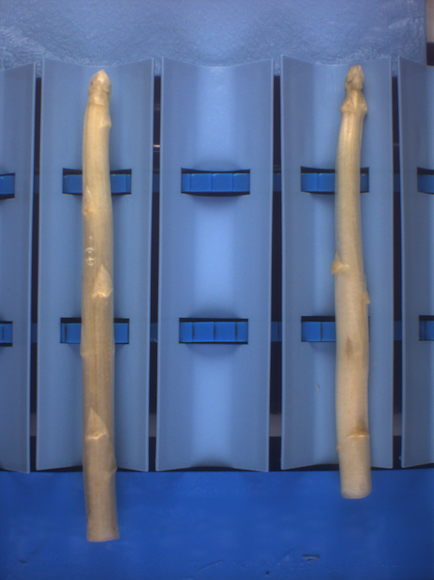
\includegraphics[width=0.9\linewidth]{Figures/chapter02/querdel_a.png}
		\caption{left}
	\end{subfigure}
	\begin{subfigure}{0.3\textwidth}
		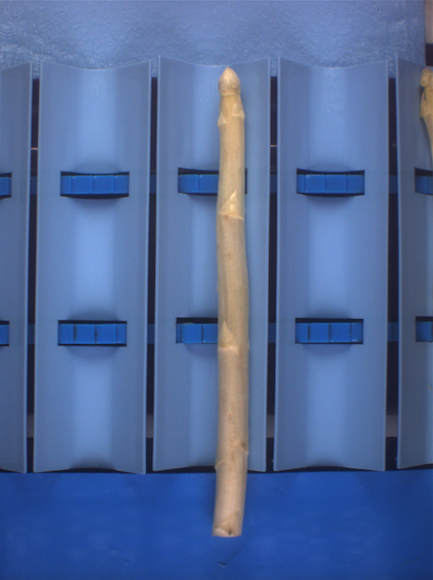
\includegraphics[width=0.9\linewidth]{Figures/chapter02/querdel_b.png}
		\caption{middle}
	\end{subfigure}
	\begin{subfigure}{0.3\textwidth}
		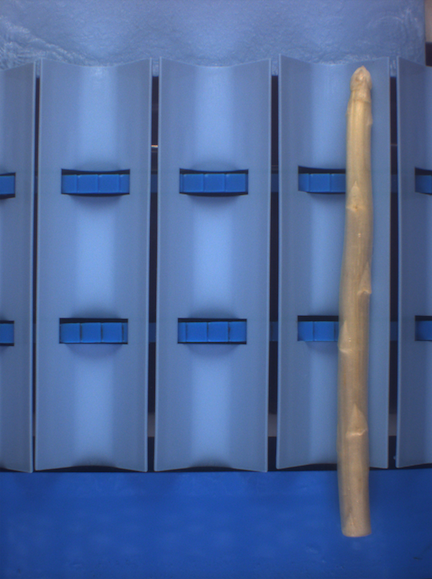
\includegraphics[width=0.9\linewidth]{Figures/chapter02/querdel_c.png}
		\caption{right}
	\end{subfigure}
	
	\begin{subfigure}{0.3\textwidth}
		\vspace{10pt}
		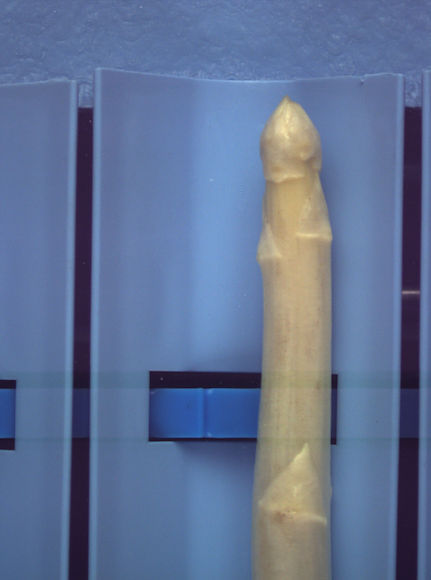
\includegraphics[width=0.9\linewidth]{Figures/chapter02/querdel_d.png}
		\caption{upper part}
	\end{subfigure}
    \caption[Example Asparagus Images Querdel's Hof]{\textbf{Example Images Querdel's Hof}~~~Example pictures of the asparagus of the farm Querdel's Hof. In picture (A), the asparagus spear is to the left, in (B), it is in the middle, and in (C) it is to the right. A fourth picture (D) is taken with a second camera with focus on the upper part of the asparagus.}
    \label{fig:ExampleImagesQuerdel}
\end{figure}

Additionally, a few images could be recorded at another asparagus farm, Querdel’s Hof, in Emsb{\"u}ren.\footnote{see~\url{https://www.querdel.de/}} The farm sorts the asparagus with an updated version of the Autoselect ATS~II at Gut Holsterfeld, that is, it uses the same software but other hardware. In particular the resolution of the camera was improved and a second camera was installed that focuses on the head region of the asparagus. At Querdel’s Hof, 20616 images were collected in total, 76 from the class label ``normal’’, 152 from the class label ``violet/flower’’, and 20388 unlabeled images. At Querdel’s Hof, each asparagus is represented by four images: three images show the asparagus from different perspectives and a fourth image depicts solely the head region. An example image can be seen in~\autoref{fig:ExampleImagesQuerdel}. No internet connection could be established to the farm, thus, no further images were collected. Moreover, the data format of the images from Querdel’s Hof is different to the data from the farm Gut Holsterfeld, due to the additional head image. Therefore a combination of both data sets was not convenient. 


\subsection{Literature research}
\label{sec:Literature}

In the classification of food products, there are numerous possibilities to apply classical machine learning and \acrshort{ann} approaches for classification tasks on image data~\citep{bhargava2018fruits,brosnan2002inspection}.

None of the found papers were suitable as blueprints for the asparagus classification project. However, some of them helped to get an idea of how to proceed with the project. For example, some papers show how the preprocessing phase could be structured~\citep{mery2013automated}, or they evaluate the machine learning methods that were already used on other food classification tasks~\citep{bhargava2018fruits}. Further, some of the literature is concerned with the classification of food products but not with differentiating between as many classes as 13~\citep{diaz2004comparison,kilicc2007classification}. Often, the variance in the food products used is either too high~\citep{zhang2012classification} or too low~\citep{kilicc2007classification,al2011dates} in comparison to the variance in our project data.  One paper evaluates the sorting of asparagus, however, it only does so on a small data set with three categories of green asparagus~\citep{donis2016classification}. Further papers on food classification are not detailed enough in their explanations and do not share the information needed for replication~\citep{pedreschi2016grading}. Another paper is mainly about the implementation of a certain toolbox~\citep{mery2013automated}.

\bigbreak
As the available data was only sparsely labeled~\citep{olivier2006semi,zhu05survey}, further research was done to evaluate the use of a semi-supervised learning approach. Details about the corresponding literature can be found in~\autoref{sec:SemiSupervisedLearning}. In regards to deep learning-based approaches, classical neural networks -- such as AlexNet, \acrshort{vgg}16/\acrshort{vgg}19, GoogleNet, Capsule Networks,  DenseNet, ResNet or \acrfull{nin} -- were assessed and presented for better understanding of the range of possible pre-trained networks and ideas for network structures~\citep{alexnet2012original,vgg2014original,googlenet2015original,capsulenet2017original,densenet2017original,resnet2016original,lin2013network}. Also, classical computer vision approaches were considered, like multiclass \acrfullpl{svm}~\citep{prakash2012multi}.
